\chapter{Anforderungen}

\section{Aufgabenstellung}
\label{sec:anforderung:aufgabenstellung}

Auf den nachfolgenden Seiten ist die unterschriebene Aufgabenstellung abgebildet.

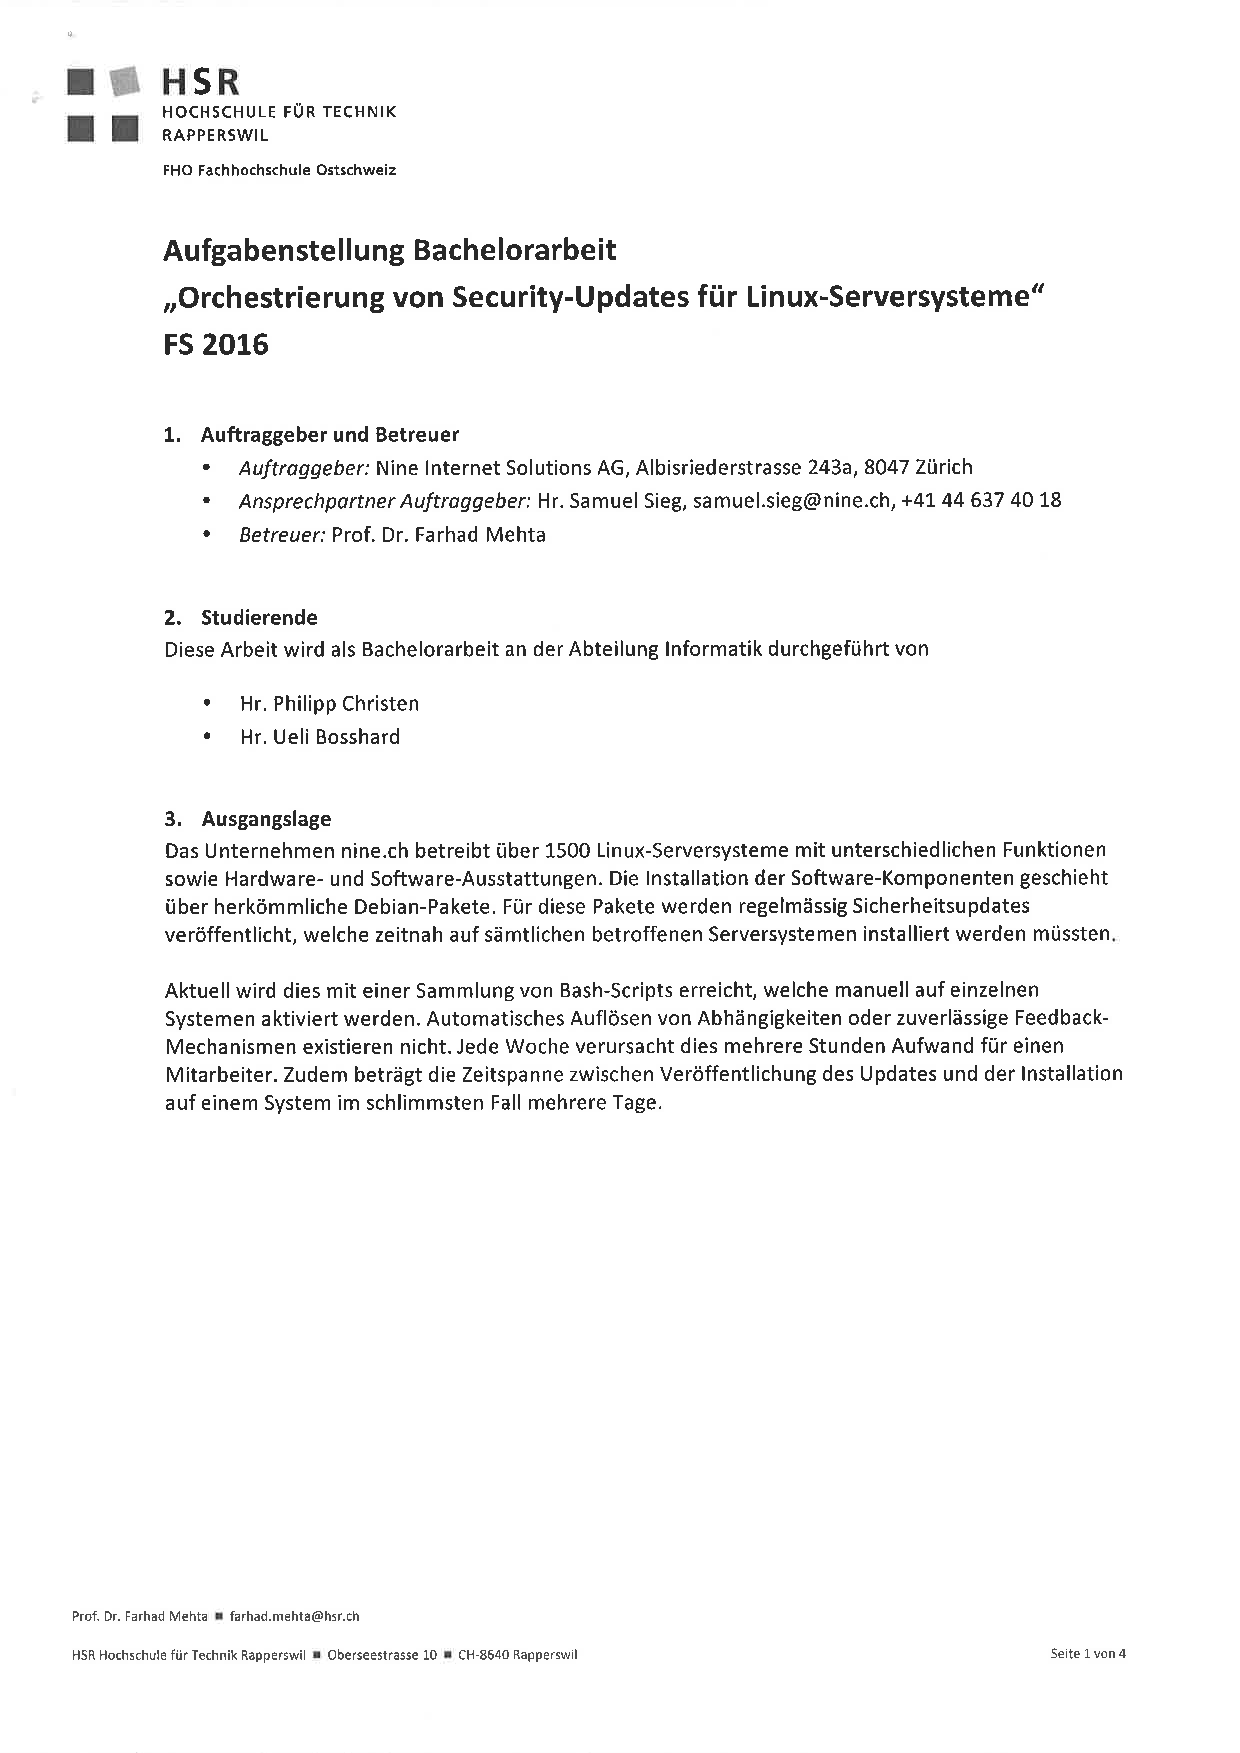
\includepdf[pages=1-,frame,scale=0.7,pagecommand={}]{files/BA_UBosshard_PChristen_SIGNED}

\begin{comment}
Ausgangslage (Kontext) und Problembeschreibung bzw. -analyse (mit Beschreibung der
Problemtyps, also ob Fokus Lösungserstellung oder Machbarkeitsanalyse). Anforderungen spezifiziert:
Funktionale Anforderungen z.B. als Use Cases (short) oder User Stories beschrieben, alle relevanten Nichtfunktionalen Anforderungen (NFA) und Qualitätsattribute abgedeckt und überprüfbar beschrieben.
\end{comment}

\section{Ausgangslage}
Die Aufgabenstellung fordert die Entwicklung einer spezifischen Software, womit sich diese Bachelorarbeit auf die Lösungserstellung fokussiert. Im folgenden sind die Anforderungen als User Stories und in den Nicht Funktionalen Anforderungen beschieben und werden im folgenden Kapitel analysiert.
\xxx[]

\section{User Stories}\label{sec:pd:user-stories}

\begin{enumerate}
    \item Als Benutzer möchte ich zu einem spezifischen System alle anstehenden Updates einsehen können, um mir schnell einen Überblick zu diesem System zu verschaffen.
    \item Als Benutzer möchte ich Systeme gruppieren können, um sie später einfacher zu finden.
    \item Als Benutzer möchte ich Pakete mehreren Paketgruppen zuordnen können, um sie später einfacher zu finden.
    \item Als Administrator möchte ich weitere Benutzer anlegen können, so dass bei meiner Abwesenheit trotzdem Updates ausgeführt werden können.
    \item Als Administrator möchte ich für Benutzer Rollen festlegen können, damit nicht jeder Benutzer einzeln konfiguriert werden muss.
    \item Als Administrator möchte ich die Rechte von Benutzergruppen auf System- und Paketgruppen-Ebene definieren können, damit ich nicht für jeden Benutzer Rechte pro System und Paket festlegen muss.
    \item Als Benutzer möchte ich auf einen Blick die wichtigsten Informationen zu all meinen Systemen sehen, damit ich sofort sehe, ob irgendwo ein Problem existiert.
    \item Als Benutzer möchte ich Pakete auf bestimmten Systemen gleichzeitig mit wenig Aufwand installieren lassen können, damit ich nicht bei jedem System einzeln anmelden muss.
    \item Als Benutzer möchte ich sehen, ob ein Agent sich seit längerer Zeit nicht mehr gemeldet hat, damit der betroffene Server nicht längere Zeit ohne Aktualisierungen auskommen muss.
    \item Als Benutzer möchte ich nach einer Auswahl von Systemen und Paketen, welche ich installieren lassen will, eine Übersicht der auszuführenden Aufgaben erhalten, damit ich prüfen kann, ob ich einen Fehler gemacht habe.
    \item Als Betreiber von Ubuntu-Servern ausserhalb der Firma \gls{nine} möchte ich, dass die Software \gls{upd89} Open Source ist, damit ich Verbesserungen oder neue Features selbst implementieren kann.
    \item Als Benutzer möchte ich, dass die Kommunikation zwischen \gls{agent} und \gls{controlcenter} verschlüsselt abläuft, damit keine \gls{mitm}-Attacken ausgeführt werden und so Angriffe gestartet werden können.
    \item Als Benutzer möchte ich sehen, wer wann auf welchen Systemen welche Updates installierte, um bei etwaigen Problemen die Ursache schnell finden zu können.
    \item Als Benutzer möchte ich im \gls{controlcenter} sehen, was \gls{apt} bei einem Updatevorgang zurückgab, damit ich mich nicht bei jedem System einzeln anmelden und die Logfiles auslesen muss.
    \item Als Administrator möchte ich neu registrierte Systeme einsehen können und diese gleich einer Systemgruppe zuweisen können, damit ich immer über neue Registrationen informiert bin.
    \item Als Benutzer möchte ich informiert werden, wenn ein Auftrag auf einem System fehlgeschlagen ist oder nicht ausgeliefert werden konnte, damit ich zeitnah prüfen kann, was mit diesem System nicht in Ordnung ist.
    \item Als Benutzer möchte ich Systeme und Pakete nach verschiedenen Kriterien filtern und sortieren können, damit ich mein gesuchtes Ziel schnell erreiche.
\end{enumerate}


\section{Nicht-funktionale Anforderungen}
%(Rahmenbedingungen, evtl. Verweis auf 1.3)

\xxx[Alle NFA/Qualitätsattribute abgedeckt und testbar beschrieben]

\subsection*{Technologien}

Anforderungen an die Technologie gehen primär aus der Aufgabenstellung hervor:

\begin{itemize}
    \item Ruby als Haupt-Programmiersprache
    \item Rails als Web-Applikations-Framework
    \item Ubuntu als unterstütztes Betriebssystem zur Verwaltung mit den Versionen 12.04 und 14.04\footnote{Ubuntu 16.04 war zu Beginn des Projektes noch nicht erschienen}
\end{itemize}

Weitere Frameworks, z.B. auf Javascript-Ebene, oder Bibliotheken werden dem Entwicklerteam überlassen.

\subsection*{Qualität}

Zusammen mit dem Industriepartner wurden folgende Nicht-funktionale Anforderungen notiert:

\begin{itemize}
\item Zuverlässigkeit: Nine.ch betreibt über 1500 Server. Diese müssen alle gleichzeitig mit dem Control Center in Verbindung stehen können.
\item Bedienbarkeit: Ein Benutzer mit durchschnittlichen Domänenkentnissen sollte in der Lage sein, die Applikation zu bedienen.
\end{itemize}